\documentclass{article}

\usepackage{graphicx}
\usepackage{amsmath,amsfonts,amssymb}
\usepackage[colorlinks,bookmarks,bookmarksnumbered,allcolors=blue]{hyperref}
\usepackage[capitalise]{cleveref}
\usepackage[top=0.75in]{geometry}
\usepackage[dvipsnames]{xcolor}
\usepackage{amsmath} 
\usepackage{esvect}
\usepackage{hyperref}
\usepackage{graphicx}
\usepackage{subcaption}
\usepackage{stfloats}
\usepackage{array}
\usepackage{booktabs}
\usepackage{amsmath}
\usepackage{caption}

\begin{document}

\author{Joe Spencer}
\title{Rotor Analysis}
\date{October 29, 2022}
\maketitle

\subsubsection*{Methods}

A rotor's performance can be computed using  \hyperlink{BEM}{blade element moment theory}. This computation makes it possible to estimate how well a rotor will perform under various conditions without having to produce and test many prototypes. The blade element momentum theory calculations for this lab were conducted using BYU FLOW Lab's \href{https://flow.byu.edu/CCBlade.jl/stable/}{CCBlade.jl} package. Used together with other julia packages, this package can calculate a rotor's \hyperlink{CP}{power}, \hyperlink{CT}{thrust}, and \hyperlink{CQ}{torque} distributions as well as its. \hyperlink{eta}{efficiency}. \newline

Some non-dimensional numbers in rotor analysis are the coefficients of power, thrust, and torque. Each of these coefficients relates a useful quantity to other known quantities including the air density, the blade diameter, and rotor's rotational velocity. Figure \ref{fig:1} shows that changing the blade diameter does not change any of these coefficients. This same result could be expected if air density or blade diameter were changed. Although the propellor would move at a different velocity and experience different forces, its coefficients would be unchanged. \newline

\begin{figure}
  \centering
  \subfloat[Power Coefficient]{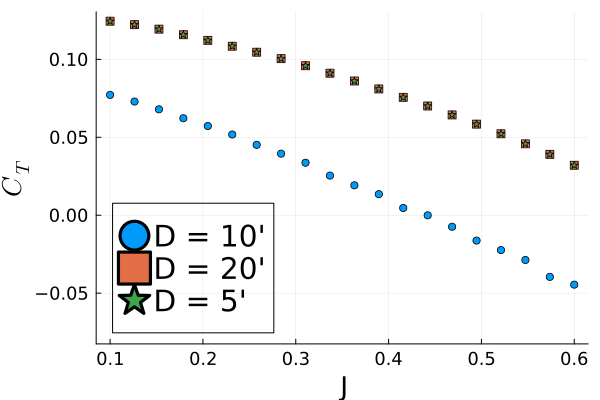
\includegraphics[width = .35\textwidth]{Plots/Figure_5.png}}
  \subfloat[Torque Coefficient]{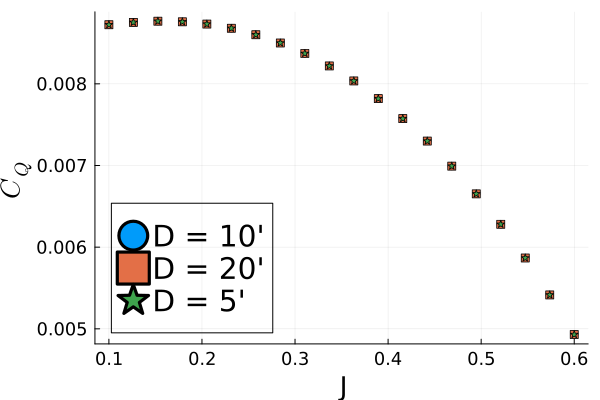
\includegraphics[width = .35\textwidth]{Plots/Figure_6.png}}
  \subfloat[Efficiency]{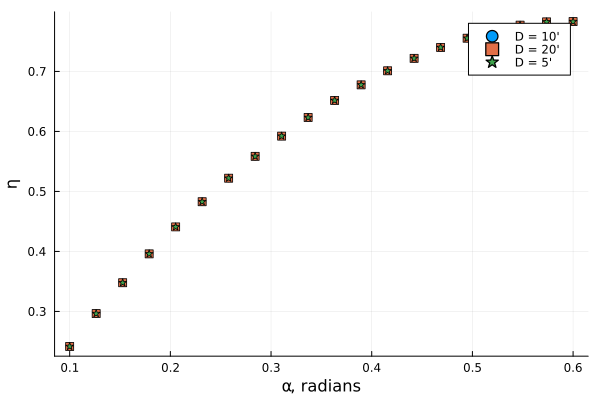
\includegraphics[width = .35\textwidth]{Plots/Figure_7.png}}
  \caption{Comparison between similar rotors of varying diameter}
  \captionsetup{aboveskip=0pt,font=it}
  \caption*{Adjusting a propellor's radius does not change the a) power or b) thrust coefficients or c) efficiency as long as its geometry remains the same.}
  \label{fig:1}
\end{figure}

Other non-dimensional constants in airfoil analysis include the \hyperlink{J}{advance ratio} and \hyperlink{lambda}{tip speed ratio}, the \hyperlink{a}{axial} and \hyperlink{a'}{tangential} induction factors, the \hyperlink{eta}{efficiency}, and the \hyperlink{sigma}{rotor solidity}. Some of these terms are closely related. For example, the tip speed ratio is simply $\pi$ divided by the advance ratio, and the power coefficient is the torque coefficient multiplied by a factor of $2 \pi$. Each number provides a benchmark reference that can relate similar airfoils under different conditions. \newline 

Since it combines two theories to obtain the power, thrust, torque, and efficiency of an airfoil, CCBlade.jl must iterate to find find them. The system of equations is iteratively solved to find the  \hyperlink{a}{axial induction factor, $a$} and \hyperlink{a'}{tangential induction factor} using an \hyperlink{phi}{inflow angle, $\phi$}. The inflow angle is then used in the third equation to find new values for $a$ and $a'$. This process is repeated until the residual between old and new values of $a$, $a'$, and $\phi$ are small enough that the user can assume they have converged to solutions. A detailed description of other variables in this system of equations can be found in the \hyperlink{BEM}{glossary}. \newline

\begin{equation}
\begin{aligned}
	\frac{1}{2} W^{2} N c C_{y} = 4 \pi U_{\infty} (1 - a) \times \Omega a' r^{2} \\
	\frac{1}{2} \rho W^{2} N c C_{x} = 4 \pi \rho [(a' \Omega r)^{2} + \Omega^{2}_{\infty} a (1 - a)] r \\
	\sin \phi = \frac{U_{\infty}}{W} (1 - a)
\end{aligned}
\end{equation}

Once these equations are solved, the axial induction factor and tangential induction factor provide the non-dimensional increase and reduction in fluid flow velocity in the normal and tangential directions to the rotor. The inflow angle provides the angle that the airfoil should form with the airflow velocity in its direction of motion to achieve this result. The system of three equations shown is possible because it combines equations from both theories. \newline

After this system of equations is solved, the solutions for $a$, $a'$, and $\phi$ are used to find $C_{P}$, $C_{T}$, $C_{Q}$ and $\eta$ for an airfoil. The user can compare these values at different inflow angles to determine which advance ratio is best for an application. Different \hyperlink{T}{twist distributions}, \hyperlink{D/D}{hub-to-tip ratios}, \hyperlink{c}{chord distributions}, and \hyperlink{APC}{propellor types} can also be investigated to compare their performances. \newline

\subsubsection*{Results and Discussion}

This research led to a few discoveries that will be useful to optimize a rotor in the next assignment. These discoveries refined the size, shape, velocity, and blade quantity of rotors and gave insights into what results from changing each variable quantity. \newline

\begin{figure}
  \centering
  \subfloat[Thrust Coefficient]{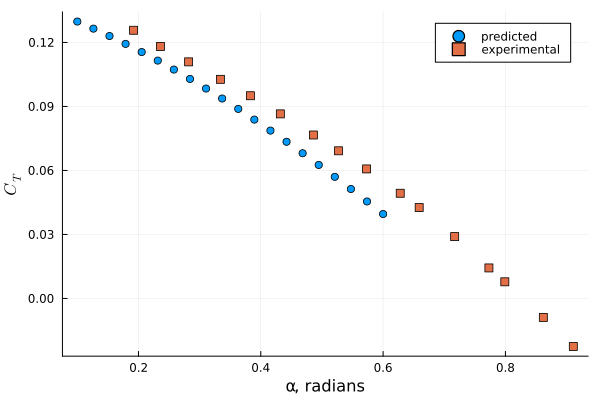
\includegraphics[width = .30\textwidth]{Plots/Figure_1.png}}
  \subfloat[Torque Coefficient]{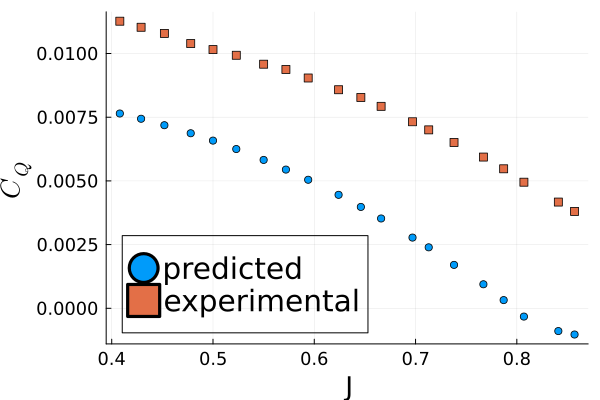
\includegraphics[width = .30\textwidth]{Plots/Figure_2.png}}

  \subfloat[Power Coefficient]{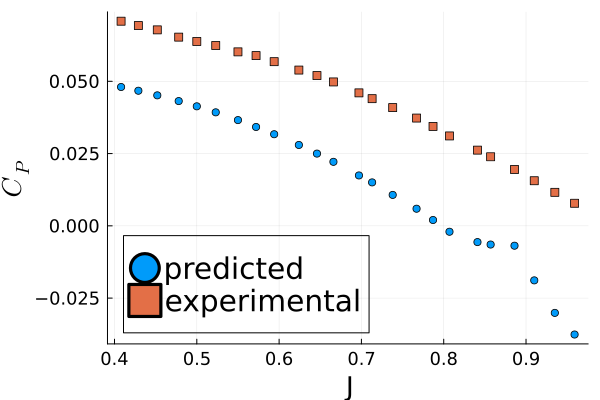
\includegraphics[width = .30\textwidth]{Plots/Figure_3.png}}\hspace{1em}
  \subfloat[Efficiency]{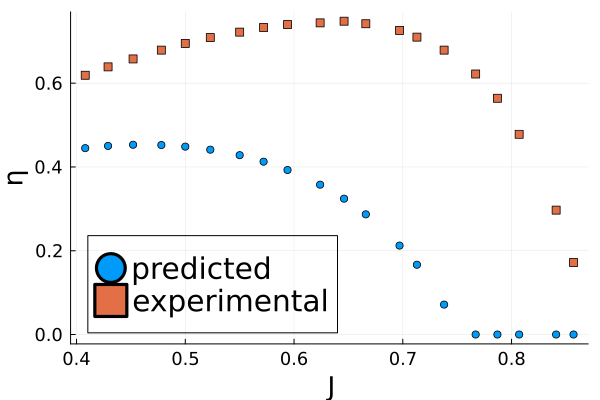
\includegraphics[width = .30\textwidth]{Plots/Figure_4.png}}
  \caption{BEM output tested against experimental data.}
  \captionsetup{aboveskip=0pt,font=it}
  \caption*{Although there are some differences, Blade Element Momentum code provides a good estimate of the constants experienced by a rotor, with error defined by the RMS calculation in equation 1. Included in this figure are comparisons between a) the thrust coefficient, b) the torque coefficient, c) the power coefficient, and d) the efficiency.}
  \label{fig:2}
\end{figure}

\textbf{1. \emph{Comparison to Experimental Data}} \newline

I first compared experimental rotor data with my own CCBlade.jl computations. CCBlade.jl has a \href{https://github.com/byuflowlab/CCBlade.jl}{github repository} containing some experimental data, which I used to test the functions I created. Figure \ref{fig:2} shows that the code found solutions close to experimental data. This is useful, because obtaining airfoil performance data in a physical experiment is very difficult. There are also many factors which could potentially invalidate these experimental results that are hard to control. \newline

A loop calculated the error using the root mean squares method. To this, it first found the average of the squared residuals by squaring each individual residual, adding the total together, and then dividing by the number of points calculated. Afterwards, the square root of this total was found, as shown in the below equation, where $y_{p}$ and $y_{a}$ are predicted and actual results. \newline

\begin{equation}
\begin{aligned}
	RMS = \sqrt{\frac{(y_{1,p}-y_{1,a})^{2} + (y_{2,p}-y_{2,a})^{2} + (y_{3,p}-y_{3,a})^{2} + ...}{N}}
\end{aligned}
\end{equation}

 The calculated errors were 28.8 percent for efficiency, 37.7 percent for the thrust coefficient, and 51.4 percent for both the thrust and torque coefficients. These were much larger than the errors calculated in the provided data, which were 9.1 percent, 7.8 percent, and 5.4 percent. This may have been do to different methods of data collection or measurement. The graphs of the torque coefficient and the pressure coefficient have the same shape. They are related by a $2 \pi$ factor. Future plots will only display the torque coefficient because of this. \newline

\begin{figure}
  \centering
  \subfloat[Thrust]{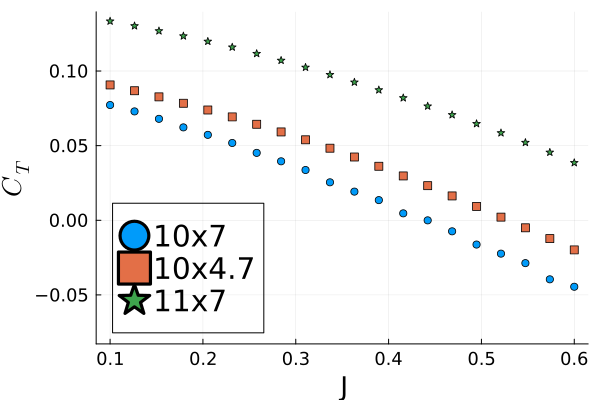
\includegraphics[width = .35\textwidth]{Plots/Figure_11.png}}
  \subfloat[Torque]{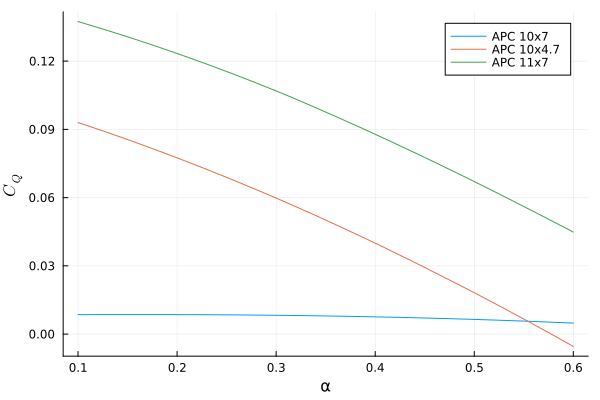
\includegraphics[width = .35\textwidth]{Plots/Figure_12.png}}
  \subfloat[Efficiency]{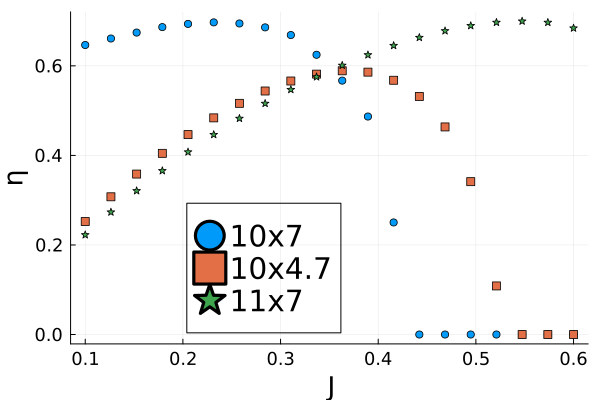
\includegraphics[width = .35\textwidth]{Plots/Figure_13.png}}
  \caption{Comparison between rotors of different length and pitch}
  \captionsetup{aboveskip=0pt,font=it}
  \caption*{Increasing a rotor's length appears to slightly increase its coefficients of thrust and torque, as shown in subfigures a) and b). Figure c) shows that decreasing a rotor's pitch dramatically decreases its efficiency at higher advance ratios.}
  \label{fig:3}
\end{figure}

\begin{figure}
  \centering
  \subfloat[Thrust]{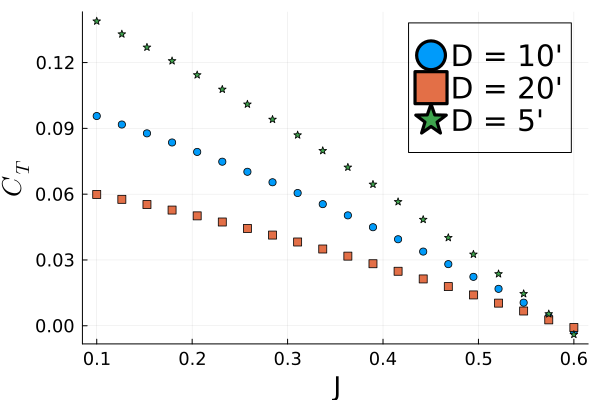
\includegraphics[width = .35\textwidth]{Plots/Figure_24.png}}
  \subfloat[Torque]{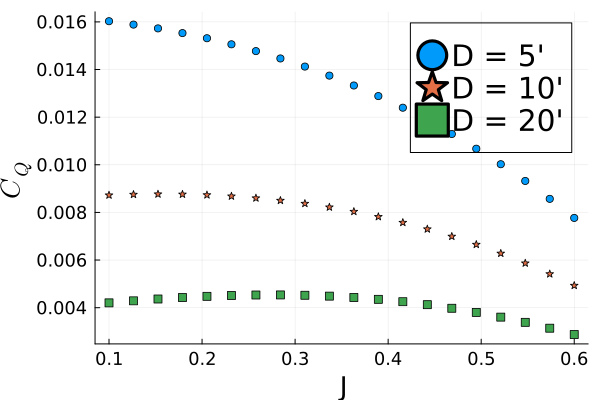
\includegraphics[width = .35\textwidth]{Plots/Figure_25.png}}
  \subfloat[Efficiency]{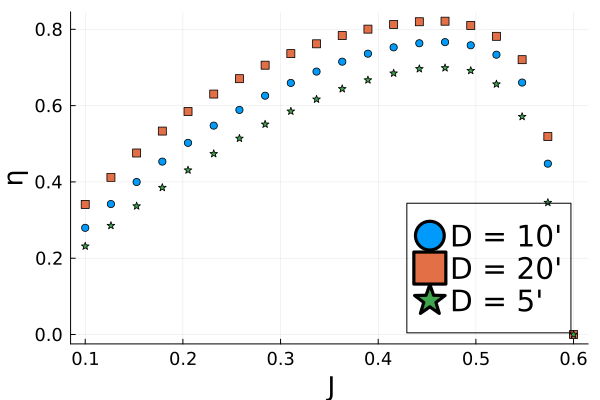
\includegraphics[width = .35\textwidth]{Plots/Figure_26.png}}
  \caption{Comparison between rotors of the same profile and thickness but different length}
  \captionsetup{aboveskip=0pt,font=it}
  \caption*{Subfigures a) and b) show that increasing the rotor blade length decreases its coefficients of both power and torque, but increases its efficiency, as seen in subfigure c).}
  \label{fig:4}
\end{figure}

\textbf{2. \emph{Radius}} \newline

As shown in figure \ref{fig:1}, the radius factor is not included in any of the non-dimensional numbers investigated in this lab. If the size of the rotor is scaled then no effect occurs. Increasing a rotor's diameter while keeping other factors the same can have an effect, though. Figure \ref{fig:3} shows a NACA 10x7 and 11x7 rotor compared to each other. The longer NACA 11x7 propellor exhibits greater coefficients of thrust and torque with a similar efficiency. \newline

Figure \ref{fig:4} shows three rotors that have the same profile, chord distribution, and chord length. Their only difference is that they are different lengths. The longest airfoil in figure 4 had the lowest coefficients of thrust and torque, but the highest efficiency. comparison between figures 1, 3, and 4 reveals that if a propellor is only magnified, then none of its coefficients are changed. If the length is increased while keeping other properties the same, then the efficiency is higher but the coefficients of thrust and torque are lower. If the pitch per revolution is decreased, then the efficiency drops at higher non-dimensional angles of attack. 

\begin{figure}
  \centering
  \subfloat[Thrust]{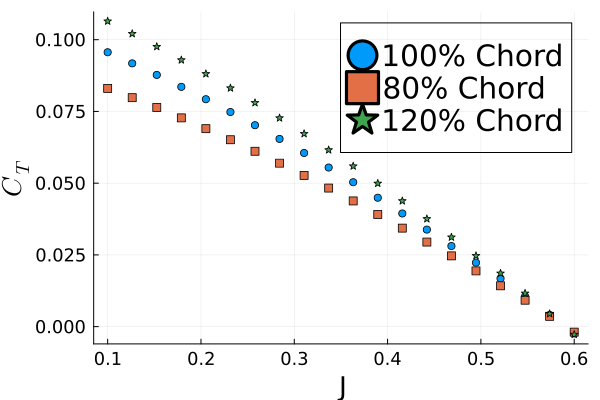
\includegraphics[width = .35\textwidth]{Plots/Figure_21.png}}
  \subfloat[Torque]{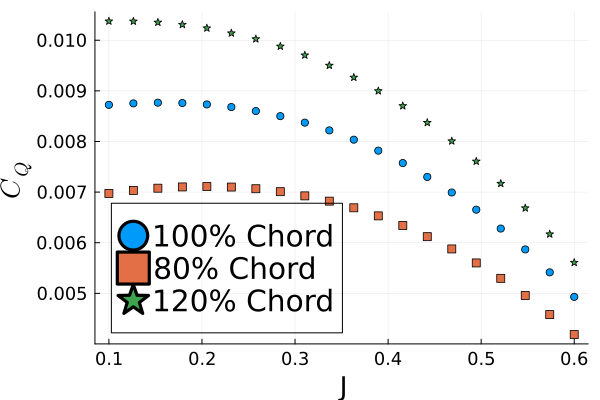
\includegraphics[width = .35\textwidth]{Plots/Figure_22.png}}
  \subfloat[Efficiency]{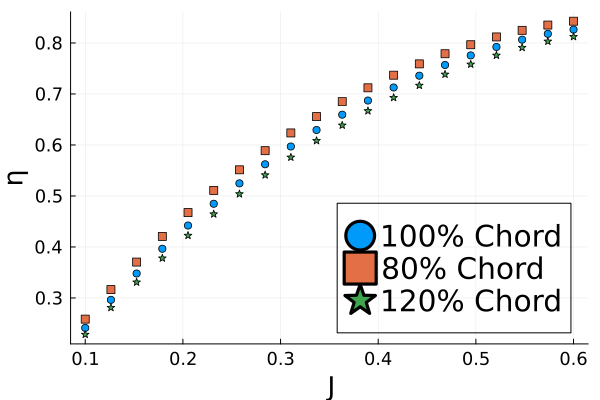
\includegraphics[width = .35\textwidth]{Plots/Figure_23.png}}
  \caption{Comparison between rotors of different chord magnitude}
  \captionsetup{aboveskip=0pt,font=it}
  \caption*{In these plots, a rotor is thickened or thinned by 20 percent. Subfigures a) and b) show that both the thrust and torque coefficients are increased when thickness is increased, while subfigure c) shows that efficiency is decreased slightly.}
  \label{fig:5}
\end{figure}

\textbf{3. \emph{Chord Distribution}} \newline

Figure \ref{fig:5} shows that increasing or decreasing a rotor's chord distribution has negative impact on its efficiency. Changing the magnitude of the chord has an enormous impact on the torque and power coefficients

\begin{figure}
  \centering
  \subfloat[Thrust]{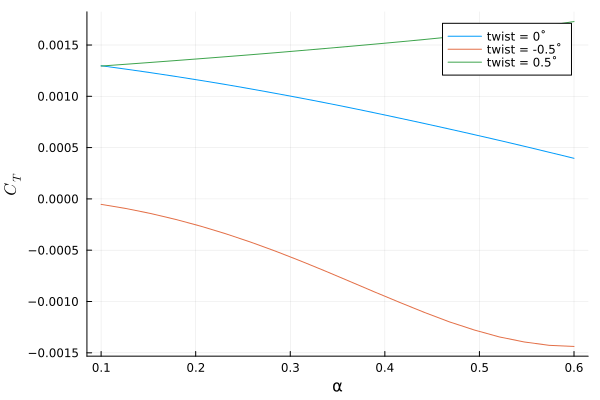
\includegraphics[width = .35\textwidth]{Plots/Figure_8.png}}
  \subfloat[Torque]{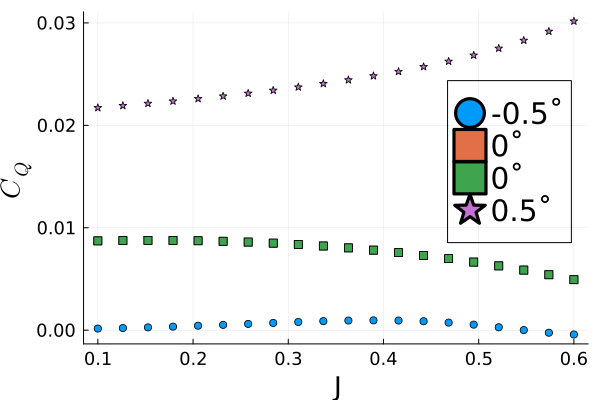
\includegraphics[width = .35\textwidth]{Plots/Figure_9.png}}
  \subfloat[Efficiency]{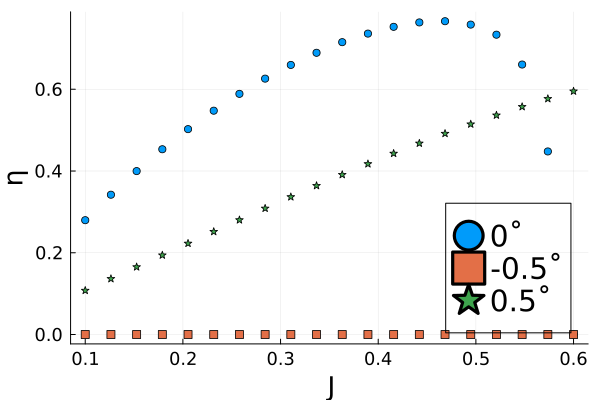
\includegraphics[width = .35\textwidth]{Plots/Figure_10.png}}
  \caption{Comparison between twist angles}
  \captionsetup{aboveskip=0pt,font=it}
  \caption*{These rotors are identical besides the angle with which they were uniformly twisted. Increasing the twist angle of a rotor increases both its thrust and torque, as seen in subfigures a) and b), while also increasing its efficiency, as in subfigure c). The rotor with the $-0.5^{\circ}$ twist angle in subfigure c) has zero efficiency at every $J$ measured, meaning that the thrust it produces is in the opposite direction of the oncoming wind.}
  \label{fig:6}
\end{figure}, though. Thickening a rotor will dramatically increase the thrust and torque coefficients. In general, to increase the thrust a rotor generates, it should be thickened. \newline

\textbf{4, \emph{Twist Distribution}} \newline

The amount a rotor is twisted can be modified so it redirects airflow and thrust differently to produces different effects. The rotor in figure \ref{fig:6} are twisted different amounts, and their thrust, torque, and efficiencies all varied significantly. The rotor with a $-0.5^{\circ}$ twist had the lowest thrust, torque, and efficiency. Its efficiency plot is at zero because the force generated by air flowing past rotor acts against its motion. In conclusion, changing a rotor's twist distribution so it is either positive or negative reduces the rotor's efficiency if it is twisted away from its optimal inflow angle. Increasing the twist angle of a rotor increases the thrust and torque coefficients, while decreasing the twist angle decreases both coefficients. \newline

\begin{figure}
  \centering
  \subfloat[Thrust]{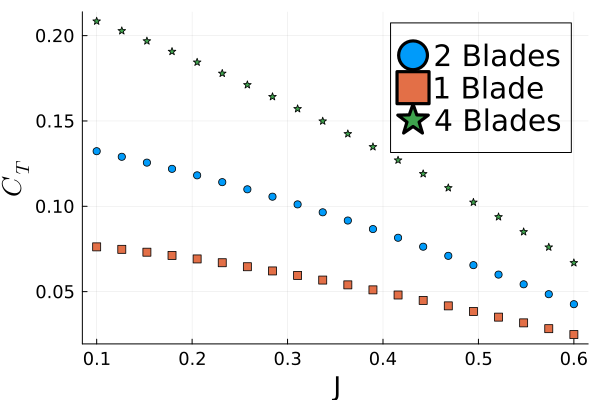
\includegraphics[width = .35\textwidth]{Plots/Figure_18.png}}
  \subfloat[Torque]{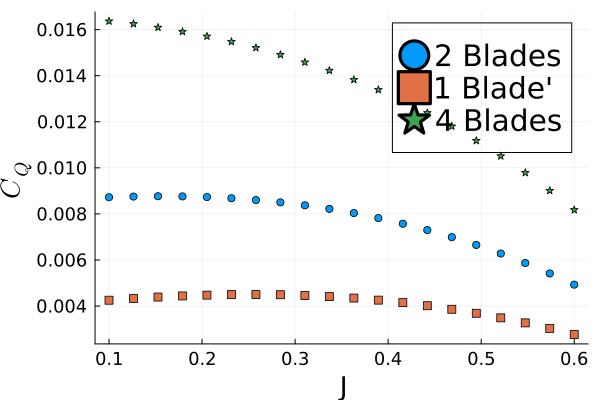
\includegraphics[width = .35\textwidth]{Plots/Figure_19.png}}
  \subfloat[Efficiency]{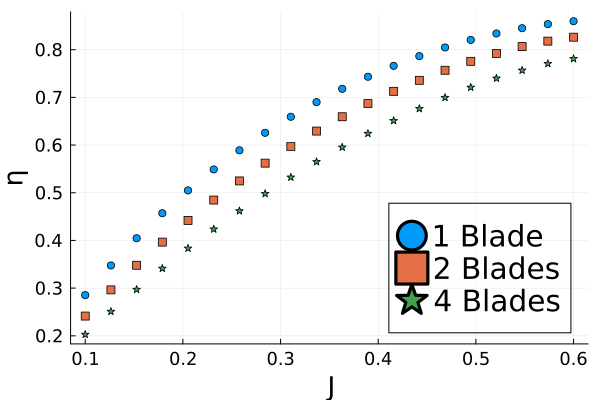
\includegraphics[width = .35\textwidth]{Plots/Figure_20.png}}
  \caption{Comparison between blade counts}
  \captionsetup{aboveskip=0pt,font=it}
  \caption*{Although thrust and torque increase with each added rotor blade, efficiency decreases. Increasing a rotor's blade count increases both its a) thrust and b) torque coefficients, but subfigure c) shows that the rotor's efficiency decreases slightly each time a blade is added to the rotor.}
  \label{fig:7}
\end{figure}

\textbf{5, \emph{Blade Count}} \newline

Increasing the number of blades in a rotor appears to increase both the thrust and torque it generates. While the thrust and torque increase, though, the efficiency decreases as the rotor's torque coefficient grows more rapidly than its thrust coefficient.

\clearpage

\section{Glossary}
\begin{itemize}
	
	\item \hypertarget{J}{Advance Ratio, $J$} - A rotor's advance ratio is a non-dimensional term. It describes the ratio how quickly a rotor is moving relative to the fluid flowing past it. A high advance ratio signifies that either the fluid is moving quickly or the rotor is moving slowly. It is described by the following equation, in which $V_{a}$ is the free stream fluid velocity, $n$ is the rotational velocity, and $D$ is the rotor diameter.
	\begin{equation}
	\begin{aligned}
		J = \frac{V_{a}}{n D}
	\end{aligned}
	\end{equation}

	\item \hypertarget{a}{Axial Induction Factor, $a$} - The axial induction factor is the ratio of the reduction in air velocity at an airfoil to its free stream velocity.
	
	\item \hypertarget{BEM}{Blade Element Momentum Theory} - The theory used to calculate local forces on a propellor or wind turbine blade. It employs both \hyperlink{BET}{blade element theory} and \hyperlink{MT}{momentum theory}. These equations are used to recursively find the \hyperlink{a}{axial induction factor, $a$}, \hyperlink{a'}{tangential induction factor, $a'$}, and \hyperlink{phi}{inflow angle, $\phi$}
	\begin{equation}
	\begin{aligned}
		\frac{1}{2} W^{2} N c C_{y} = 4 \pi U_{\infty} (1 - a) \times \Omega a' r^{2} \\
		\frac{1}{2} \rho W^{2} N c C_{x} = 4 \pi \rho [(a' \Omega r)^{2} + \Omega^{2}_{\infty} a (1 - a)] r \\
		\sin \phi = \frac{U_{\infty}}{W} (1 - a)
	\end{aligned}
	\end{equation}
In these equations, $a$, $a'$, and $\phi$ are the previously mentioned axial and tangential induction factors and inflow angle. The airfoil's inflow velocity is represented by the letter $W$, $N$ is the number of propellers, $\rho$ is the fluid density, $c$ is the chord length, $C_{x}$ and $C_{y}$ are obtained by the equation below, $U_{\infty}$ is the fluid free velocity, $\Omega$ is the blade's angular speed, and $r$ is the radius to the tip of the blade.
	\begin{equation}
	\begin{aligned}
		C_{x} = c_{l} \cos{\phi} + c_{d} \sin{\phi} \\
		C_{y} = c_{l} \sin{\phi} + c_{d} \cos{\phi}
	\end{aligned}
	\end{equation}
	
	\item \hypertarget{BET}{Blade Element Theory} - Blade element theory calculates the forces on a turbine blade by dividing it into finite pieces and summing the forces on all of these pieces. This theory determines the induced velocity and efficiency of a point along a blade using these equations:
	\begin{equation}
	\begin{aligned}
		v_{i} = \sqrt{\frac{T}{A} \frac{1}{2 \rho}} \\
        		\eta = \frac{\tan{\phi}}{\tan{(\phi + \gamma)}}
	\end{aligned}
	\end{equation}
In these equations, $v_{i}$ is the uniform induced velocity across the disk, $T$ the thrust it experiences, $A$ is its area, $\rho$ is the air density, $\phi$ is the angle to the airfoil's plane of rotation as it moves forward, and $\gamma$ is the difference between $\phi$ and $\beta$, what the airfoil's actual inflow angle would be if it were stationary.

	\item \hypertarget{c}{Chord Distribution} - The chord length distribution shows the length of a rotor's chord at different angular positions around itself. An airfoil with a constant angle of attack $\alpha$ as it generates lift has an elliptic chord distribution.
	
	\item \hypertarget{CP}{Coefficient of Power, $C_{P}$} - A propellor's coefficient of power signifies how efficient a wind turbine is. It is the ratio of the power generated by a wind turbine to the total power of the wind flowing through it. The power generated or absorbed by an airfoil can be described by the following equation, where $P$ is power, $C_{P}$ is the coefficient of power, $\rho$ is fluid density, $n$ is the velocity in revolutions per second, and $D$ is the propellor diameter. The power coefficient and the \hyperlink{CT}{torque coefficient} are proportional to each other by a factor of $2\pi$.
	\begin{equation}
	\begin{aligned}
		P = \rho n^{3} D^{5} C_{P} \\
		C_{P} = 2 \pi C_{Q}
	\end{aligned}
	\end{equation}
	
	\item \hypertarget{CT}{Coefficient of Thrust, $C_{T}$} - A rotor's thrust coefficient determines how much thrust in the forward direction an airfoil experiences. Thrust force is directly opposite drag. Please note the similarities and differences between the thrust equation and the \hyperlink{CP}{power equation}.
	\begin{equation}
	\begin{aligned}
		T = \rho n^{2} D^{4} C_{T}
	\end{aligned}
	\end{equation}
	
	\item \hypertarget{CQ}{Coefficient of Torque, $C_{Q}$} - A rotor's torque coefficient defines how much torque it will experience. A propellor's torque is given by the following equation, in which $Q$ represents torque, $\rho$ is the fluid density, $n$ is the velocity in revolutions per second, $D$ is the diameter, and $C_{Q}$ is the coefficient of torque. The torque coefficient and the \hyperlink{CP}{power coefficient} are proportional to each other by a factor of $2\pi$.
	\begin{equation}
	\begin{aligned}
		Q = \rho n^{2} D^{5} C_{Q} \\
		C_{Q} = \frac{C_{P}}{2 \pi}
	\end{aligned}
	\end{equation}
	
	\item \hypertarget{eta}{Efficiency, $\eta$} - A rotor's efficiency can be described by the following equation, in which $J$ is the rotor's \hyperlink{J}{advance ratio}, $C_{T}$ is its \hyperlink{CT}{thrust coefficient}, and $C_{P}$ its \hyperlink{CP}{power coefficient}:
	\begin{equation}
	\begin{aligned}
		\eta = J \frac{C_{T}}{C_{P}}
	\end{aligned}
	\end{equation}
	
	\item \hypertarget{D/D}{Hub-to-Tip Ratio} - A rotor's hub-to-tip ratio divides the distance along the blade that is actually exposed wind by the entire length of the blade. This needs to be taken into account when calculating constants like the airfoil's \hyperlink{lambda}{tip speed ratio}.
	
	\item \hypertarget{phi}{Inflow angle, $\phi$} - The inflow angle, sometimes denoted by the Greek letter $\phi$, is the angle between the freest stream velocity and the velocity of the airfoil as it rotates. It is used in \hyperlink{BEM}{blade element momentum theory} calculations.
	
	\item \hypertarget{MT}{Momentum Theory} - Momentum theory defines the power required to produce sufficient thrust to maintain momentum in a blade by the following equation, where $T$ is thrust, $\rho$ is density, $A$ is disc area, and $P$ is power:
	\begin{equation}
	\begin{aligned}
        		P = \sqrt{\frac{T^{3}}{2 \rho A}}
	\end{aligned}
	\end{equation}
	
	\item \hypertarget{APC}{Propellor Identification} - A propellor is identified by 2 numbers, which represent its diameter and its pitch, both in inches. For example, an APC 10x7 propellor is made by Advanced Precision Composites. It has a 10-inch diameter and a 7-inch pitch per revolution.
	
	\item \hypertarget{sigma}{Rotor Solidity, $\sigma$} - Rotor solidity describes the ratio of a turbine's chord length, $c$, to its spacing, $s$. This is found by the following equation, in which $n_{b}$ is the number of blades, $r_{h}$ is the hub radius, and $r_{t}$ is the tip radius.
	\begin{equation}
	\begin{aligned}
		\sigma = \frac{c}{s} = \frac{c n_{b}}{2 \pi \sqrt{\frac{r^{2}_{h} + r^{2}_{t}}{2}}}
	\end{aligned}
	\end{equation}
	
	\item \hypertarget{a'}{Tangential Induction Factor, $a'$} - The tangential induction factor is the ratio of the increase in air velocity tangential to the airfoil to its free stream velocity.
	
	\item \hypertarget{lambda}{Tip Speed Ratio, $\lambda$} - A wind turbine's tip speed ratio is the inverse of its \hyperlink{J}{advance ratio, $J$}. It represents the ratio of the speed of the tip of a turbine blade, or $\omega R$, to the wind speed, $v$.
	\begin{equation}
	\begin{aligned}
		\lambda = \frac{\omega R}{v} = \frac{\pi}{J}
	\end{aligned}
	\end{equation}
	
	\item \hypertarget{T}{Twist Distribution} - Twist distribution along a wing redirects where air flows past it. This causes changes in both the magnitude and location lift and drag forces it experienced as air flows past it.
	
\end{itemize}

\end{document}